\documentclass[namedate,webpdf,contemporary,large]{TBench-template}
\usepackage[english]{babel}
\usepackage{graphicx}
\usepackage{amsmath}
\begin{document}
\journaltitle{BenchCouncil Transactions on Benchmarks, Standards and Evaluations}
\DOI{}
\appnotes{Research Article}
\firstpage{1}
\title[Label coverage bounds]{Label Coverage Bounds Pooled Macro F1: A Reporting Diagnostic for Closed-Set IDS Benchmarks}
\author{Author withheld for review}
\authormark{Anonymous submission}
\abstract{We present a pre-fit audit of the label outputs a benchmark split permits. On the original-label NSL-KDD split, reaggregating the same five forest confusion matrices from fine labels to five categories raises mean macro F1 from 0.23953 (SD 0.00878) to 0.48349 (SD 0.00549), while the ceiling changes from 0.55263 to 1. A corrected CICIDS2017 Friday holdout has a fine-label ceiling of 0.20 because only BENIGN occurs in both train and test vocabularies. We re-score ten confusion matrices from one openly released study and find its result compatible with a ceiling of one. No incompatible published score is verified. The findings support reporting legal outputs and scoring conventions but do not establish field-wide impact. Code, counts and split manifests accompany the paper.}
\keywords{Macro F1, label coverage, benchmark protocols, intrusion detection, reproducibility}
\maketitle

\section{Introduction}
A low benchmark score can describe two different failures: a model misclassifies a label it can output, or the evaluation asks it to name a label outside its output vocabulary. These failures have different remedies. Better features or fitting might address the first. They cannot address the second without changing the model's permitted decisions.

NSL-KDD provides a natural example: 21 of the 38 fine-grained labels in its official test set occur in training. A classifier restricted to training labels therefore has a positive-test-support ceiling of 21/38 (0.55263). CICIDS2017 leave-one-day-out is more extreme: its 14 attack labels are each confined to one capture day, giving a 15-class ceiling of 1/15. The attack schedule is known; this paper records the scoring consequence under an explicit label inventory.

The coverage inequality follows directly from recall and precision; we do not present it as a new theory of F1. The contribution is an operational audit for pooled scoring when legal vocabularies differ across folds: it computes the fraction of each class's test rows that can be named, makes the chosen output inventory explicit, and distinguishes training-restricted models from global-head and open-set tasks. We add a paired label-resolution analysis on NSL-KDD and a source-based audit of published evaluation practice. The broader search has not established a published score that violates its legal-output ceiling, so impact on prior reported conclusions remains unproven. An optional vocabulary oracle accounts for false positives sent to legal destinations; its proofs and computational details are in the supplement.

The empirical examples illustrate how the same fixed predictions score under different label inventories. These are different tasks, so score differences are descriptive rather than evidence that one model is better. In a published NSL-KDD study, Ayantayo et al. describe 17 test-only fine-grained attack types, map the task to five broad categories, and also construct a test subset without those unseen subtypes \cite{ayantayo2023}. Under that five-category output space, the five categories are available in training and the ceiling is one; the reported category task does not establish fine-grained attribution of unseen subtypes. This is a verified example of target resolution in published practice, not an incompatible score. Our broader frozen screen still establishes no published score conflict.

\section{Related Work}
Security evaluations can become misleading when the sampling protocol answers a different question from the intended deployment setting \cite{sommer2010,arp2022}. Dataset surveys and CICIDS2017 audits document traffic-generation, feature and labeling limitations \cite{ring2019,engelen2021,lanvin2023}. We condition on the released labels and a declared partition; the present analysis neither repairs those datasets nor removes their other biases.

Macro F1 itself requires an explicit definition. Averaging class F1 differs from taking the harmonic mean of macro precision and recall \cite{opitzburst2019}. Pooling out-of-fold predictions also differs from averaging fold scores \cite{forman2010}. Work on classification metrics studies prevalence and prediction bias \cite{opitz2024,sokolova2009}, while confusion-matrix objectives can guide learning algorithms \cite{narasimhan2015}. Our optimization uses the true test labels to bound a fixed evaluation cohort; it is not a learning procedure.

Label shift concerns changed class priors under assumptions on conditional feature distributions \cite{lipton2018}. A missing legal output is a separate constraint: reweighting cannot create that output. Open-set recognition and selective prediction add unknown or reject decisions \cite{scheirer2013,geng2021,chow1970,geifman2019}. Generalized zero-shot learning permits unseen outputs through side information and evaluates seen and unseen recognition separately \cite{xian2017}. These settings explain why absence from training alone is insufficient to establish zero recall. Temporal and spatial discipline, as in TESSERACT \cite{pendlebury2019}, remains necessary even when every legal label is covered.

\section{A Score Limit from Legal Outputs}
Let \(f\) index folds, \(T_f\) their training labels, and \(V_f\ne\varnothing\) their legal output vocabularies. Assume a nonempty pooled test cohort. Every test row receives one label in \(V_f\). We allow \(V_f\) to contain labels absent from \(T_f\); training-restricted classifiers are the special case \(V_f=T_f\). Write \(n_{fk}\) for fold-level test support and define
\[
\begin{aligned}
S&=\{k:\textstyle\sum_f n_{fk}>0\},\quad n_k=\sum_f n_{fk},\\
m_k&=\sum_fn_{fk}\mathbf{1}\{k\in V_f\},\quad \rho_k=m_k/n_k\ (k\in S).
\end{aligned}
\]
The primary metric pools confusion counts and averages F1 over positive-test-support labels \(S\). We also report the inferred union of true and predicted labels, the default label inventory when scikit-learn's \texttt{f1\_score} is called without an explicit \texttt{labels} argument. These conventions can differ when a legal output has no test support. Train-only or other output-only labels remain in the vocabulary input for both calculations.

\paragraph{Proposition 1. Coverage ceiling.}
Every legal prediction vector satisfies
\[
F\le C=\frac{1}{|S|}\sum_{k\in S}\frac{2\rho_k}{1+\rho_k}.
\]
\emph{Proof.} A true positive needs a legal true label, hence \(TP_k\le m_k\) and recall is at most \(\rho_k\). Precision is at most one. Substitution in the increasing harmonic-mean expression for F1 proves the result. Equality needs every available row correct and no false positives entering a positive-\(m_k\) class.

Support-weighted F1 replaces \(1/|S|\) with \(n_k/\sum_jn_j\). Micro F1, with all true and predicted labels included, equals accuracy and is at most \(\sum_km_k/\sum_kn_k\). Balanced accuracy is at most \(|S|^{-1}\sum_k\rho_k\). These are deterministic cohort limits, not confidence intervals.

For leave-one-group-out using all remaining groups as training and \(V_f=T_f\), a label in one group has \(\rho_k=0\); a label in two or more groups has \(\rho_k=1\). Thus fractional pooled coverage requires another structure, such as a forward or restricted-window protocol. This explains both the severity and the simple form of the CICIDS2017 result.

\subsection{Legal outputs and limited training support}
A global head permitting every test label has \(C=1\), including when some labels have no training examples. This is the correct legal ceiling. It is not evidence that the missing classes can be learned. There is no distribution-free improvement based only on training counts: a feature can encode its correct global label, and a fixed classifier can decode it perfectly without any examples of that label. Conversely, the same counts can accompany uninformative features.

For sensitivity analysis, define \(V_f(\tau)=\{k:N^{\mathrm{train}}_{fk}\ge\tau\}\). Recomputing the bound describes how coverage changes with a declared support requirement. It is a hard ceiling only for a model that enforces this restricted vocabulary. Calling it a learnability ceiling for unrestricted networks would require additional assumptions about features, priors, side information and learning. The package therefore accepts legal vocabularies explicitly and uses training labels only as the default.

\section{Vocabulary Oracle}
The coverage ceiling counts unavailable true labels but assumes all available rows are classified correctly and creates no false positives. The exact vocabulary oracle \(O\) is the maximum pooled macro F1 under perfect classification of available rows and optimal legal destinations for unavailable rows; it includes false positives created by those destinations. When exact optimization is not run, the sandwich bounds \(L\le O\le U\) use the sum and the maximum of the foldwise minimum destination costs, respectively. These quantities describe attainable-score limits, not model performance; their derivation and the grouped solver are in the supplement.

\section{Evaluation Design}
The main experiments use CICIDS2017 \cite{sharafaldin2018} and original-label NSL-KDD \cite{tavallaee2009}. Counts, input hashes, membership manifests and confusion matrices accompany the code. Primary results use pooled positive-test-support macro F1 and source-training-label outputs; the NSL pipeline comparison also reports inferred-union scores. CIC forests use 100 trees. Seeds 42--46 describe initialization variation on fixed cohorts, not independent networks or test sets. Additional UNSW-NB15 and gas-sensor analyses are reported in the supplement.

We separately use the corrected DistriNet CICIDS2017 release, which supplies timestamped per-day CSVs and revised labels \cite{engelen2021,lanvin2023}. Monday through Thursday form the training pool and Friday is the chronological test day. Flow identifiers, endpoint addresses and ports, timestamp, and label are excluded from features. We cap the training sample at 5,000 rows per observed label and seed (35,603 rows in the realized sample); all 21 training labels remain represented. Random Forest, Extra Trees, and SGD with log loss are each run with seeds 42--44 on the same full Friday cohort. These fits quantify model variation on this fixed split; they are not independent tests or a comparison isolating the effect of corrected labels.

CICIDS2017 compares five-fold stratified shuffled cross-validation with capture-day holdout. Numeric imputation uses training medians; web-label spelling variants are normalized. The local MachineLearningCVE CSVs contain no timestamps. A historical within-day row-order result is retained in the artifact but is not described as a verified temporal cutoff. All six archived forest configurations, including bootstrap weighting and that historical split, have separate fresh replication records agreeing with archived metrics to \(10^{-12}\).

NSL-KDD uses its named training and test files. Randomized pipelines were fit with seeds 42--46. GaussianNB and kNN are deterministic under these settings; GaussianNB was refit five times and kNN's identical deterministic predictions were reused. The forest retains its existing one-hot encoding; the five added pipelines use one-hot nominal encoding and training-fitted numeric standardization. The comparison therefore concerns complete pipelines, not isolated estimators.

\section{Results}
\subsection{NSL-KDD: a natural partial-coverage split}
Of the 38 test labels, 17 are unavailable to a training-restricted classifier. The positive-test-support ceiling and oracle are 0.55263. Two train-only labels can receive predictions without adding a class to that score's denominator. Under inferred-union scoring those destinations are scored as zero-F1 classes, and the exact oracle is 0.54837. Across five forest seeds, mean full-cohort F1 is 0.23953 (SD 0.00878); no unavailable test label is correctly predicted. The constraint is material to the attainable score, while model errors account for a large remaining gap.

The five-category mapping has ceiling one. This does not repair fine-grained recognition; it asks whether the system identifies a broader category. Reporting a high category score and a low fine-label score as interchangeable evidence would obscure this distinction.

\begin{table}[h]\centering
\caption{NSL-KDD forest scores on the same official test rows. Covered scoring removes unavailable rows and changes the scored label set.}
\begin{tabular}{rrr}
Seed & Full support-scored F1 & Covered support-scored F1\\
42 & 0.25456 & 0.48702\\
43 & 0.23488 & 0.45491\\
44 & 0.23764 & 0.45548\\
45 & 0.23850 & 0.45566\\
46 & 0.23205 & 0.45612\\
\end{tabular}\end{table}
These five fits share one training file and one test file. Full scores range from 0.23205 to 0.25456; covered scores range from 0.45491 to 0.48702. We report the seed range as fit variation on this fixed cohort and do not interpret the small seed-level order changes as ranking stability or population uncertainty.

\paragraph{Prespecified pipeline comparison.}
We compare all six prespecified pipelines on the same official NSL-KDD split. For the four randomized pipelines, table entries are means and standard deviations over seeds 42--46. GaussianNB and kNN are deterministic under these settings; each has one distinct prediction matrix, so their SD across the five seed labels is zero. GaussianNB was refit five times and kNN's identical deterministic predictions were reused. The forest and added pipelines use different preprocessing, so these results compare complete pipelines rather than estimator families. Full and covered-row scores target different label inventories; neither is a substitute for the other.
\begin{table}[h]\centering
\caption{NSL-KDD pipeline scores under positive-test-support scoring. Values are mean $\pm$ SD across five declared seeds.}
\begin{tabular}{lrr}
Pipeline & Full F1 & Covered F1\\
Random forest & 0.23953 $\pm$ 0.00878 & 0.46184 $\pm$ 0.01409\\
Extra Trees & 0.22314 $\pm$ 0.00162 & 0.45095 $\pm$ 0.00048\\
Decision tree & 0.24664 $\pm$ 0.00825 & 0.50294 $\pm$ 0.00985\\
Gaussian NB & 0.17968 $\pm$ 0.00000 & 0.34711 $\pm$ 0.00000\\
SGD logistic & 0.20319 $\pm$ 0.01521 & 0.40073 $\pm$ 0.02966\\
kNN & 0.25160 $\pm$ 0.00000 & 0.53995 $\pm$ 0.00000\\
\end{tabular}\end{table}
\begin{table}[h]\centering
\caption{The same NSL-KDD predictions scored over the inferred union of true and predicted labels. Values are mean $\pm$ SD.}
\begin{tabular}{lrr}
Pipeline & Full F1 & Covered F1\\
Random forest & 0.23338 $\pm$ 0.00855 & 0.44084 $\pm$ 0.01345\\
Extra Trees & 0.21742 $\pm$ 0.00158 & 0.43046 $\pm$ 0.00046\\
Decision tree & 0.24032 $\pm$ 0.00803 & 0.48007 $\pm$ 0.00940\\
Gaussian NB & 0.17507 $\pm$ 0.00000 & 0.33133 $\pm$ 0.00000\\
SGD logistic & 0.19588 $\pm$ 0.01274 & 0.37548 $\pm$ 0.02235\\
kNN & 0.24515 $\pm$ 0.00000 & 0.51540 $\pm$ 0.00000\\
\end{tabular}\end{table}
Among these six complete pipelines, kNN has the highest point estimate under both scoring conventions. On full positive-support scoring, its 0.25160 mean is 0.00496 above the decision tree's 0.24664, smaller than the tree's 0.00825 seed SD; kNN is deterministic here, so this comparison does not quantify model-to-model uncertainty. On covered rows its mean lead over the tree is 0.03701, while the covered-row task remains conditional and differs from full scoring. These results do not isolate estimator effects or establish a general performance ranking.

We also reaggregate each saved forest confusion matrix to the dataset's five broad categories without refitting. The fine-label mean remains 0.23953 (SD 0.00878) under a ceiling of 0.55263; the projected five-category mean is 0.48349 (SD 0.00549) under a ceiling of 1. The 3,750 rows carrying unavailable fine labels map to categories present in training. This paired calculation makes the role of label resolution concrete: category-level scoring accepts correct family predictions even when the exact attack subtype is unavailable. It is not a comparison between separately trained fine- and coarse-label models. The release records the full mapping for the 40-label train/test union; 38 labels have positive test support. For an operational mixed-resolution score, every attack family containing a test-only subtype must be grouped for both truth and prediction. All four NSL-KDD attack families contain at least one such subtype, so this coherent mixed taxonomy is identical to the five-category task above. Its inferred-union and positive-support scores are therefore equal at 0.48349 (SD 0.00549): all five output categories have positive test support, and the predictions map only to those five categories. It does not isolate a score change for only the 17 unavailable rows; changing their resolution alone while retaining fine labels for sibling attacks would not define one fixed output taxonomy for both truth and prediction.

\begin{table}[h]\centering
\caption{Label resolution changes the score and ceiling for the same five saved NSL-KDD forest prediction matrices. Both true and predicted labels are mapped to the five categories.}
\begin{tabular}{lrr}
Target & Ceiling & Macro F1, mean $\pm$ SD\\
Fine attack subtype & 0.55263 & 0.23953 $\pm$ 0.00878\\
Five attack categories & 1.00000 & 0.48349 $\pm$ 0.00549\\
\end{tabular}\end{table}

\subsection{CICIDS2017: a day holdout changes the scoring task}
Every attack class appears on one day. Benign traffic remains available whenever tested, giving \(\rho_{\mathrm{BENIGN}}=1\); the 14 attack fractions are zero. Hence \(F=F_{\mathrm{BENIGN}}/15\) and \(C=O=0.06667\). The unweighted forest's score changes from 0.85347 in shuffled cross-validation to 0.06030 in day holdout. Under the latter protocol the attack F1 terms are fixed at zero, so their contribution cannot distinguish these training-restricted classifiers.

\begin{figure}[h]\centering
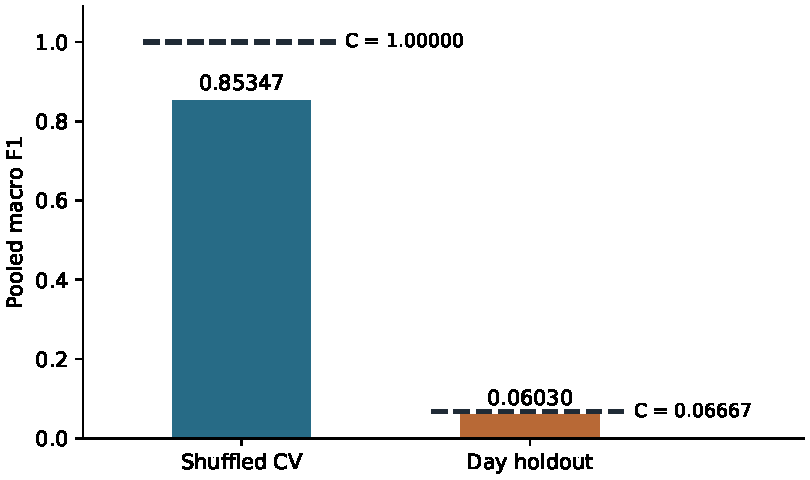
\includegraphics[width=0.95\columnwidth]{figures/cic_hero.pdf}
\caption{CICIDS2017 unweighted forest. Shuffled cross-validation has full label coverage; day holdout makes all fine-grained attack labels unavailable. The ceiling is a property of each protocol.}
\end{figure}

The day-held-out unweighted forest has benign recall 0.99858. Of the 557,646 unavailable attack rows, 475,727 are sent to benign and the remainder to other attack labels. Those other attack labels have zero covered support in the pooled score, so they provide free oracle destinations. This explains why the exact oracle equals the coverage ceiling here. The micro ceiling is 0.80300 because benign dominates the cohort. Merging web labels gives a 13-label ceiling of 0.07692; the declared eight-family mapping gives 0.25; binary attack detection has ceiling one. These are different evaluation targets.

\subsection{Corrected CICIDS2017: Friday labels are unavailable after earlier-day training}
The corrected release contains 1,552,899 Monday--Thursday training rows and 547,915 Friday test rows. Its five test-positive labels are BENIGN, Bot, Bot - Attempted, DDoS, and PortScan. Only BENIGN occurs in the training vocabulary, so all four attack-label recalls are zero for any classifier restricted to observed training labels; the fine-label ceiling is C = 1/5 = 0.20. This is a result on the corrected, timestamped release and a separate split from the original-release LODO analysis above.

On the fixed Friday cohort, mean positive-support macro F1 is 0.15513 (SD 0.00168) for Random Forest, 0.15542 (SD 0.00122) for Extra Trees, and 0.17464 (SD 0.00728) for SGD log loss. The per-class training cap changes class priors, and model-specific calibration and thresholds also differ. We report these as fixed settings, not as a model-quality comparison. The cap and label variants affect fitting; this experiment does not estimate the isolated effect of relabeling because no matched old-release fit is included.

\begin{table}[h]\centering
\caption{Corrected CICIDS2017 Friday holdout: means and sample SDs over three seeds on one fixed test cohort. The attainment ratio F/C is about 0.78--0.87 but mostly reflects benign-class F1; it is not attack-detection quality. Binary scores appear in the summary table below.}
\label{tab:corrected-cic}
\begin{tabular}{p{4.2cm}p{3.3cm}rr}
Model setting & Fine macro F1 & Ceiling (C) & (F/C) \\
Random Forest & 0.15513 (0.00168) & 0.20000 & 0.77566 \\
Extra Trees & 0.15542 (0.00122) & 0.20000 & 0.77708 \\
SGD log loss & 0.17464 (0.00728) & 0.20000 & 0.87320 \\
\end{tabular}\end{table}

The same unit ceiling can accompany very different attack detection. The summary table collects the binary results once; C = 1 in each row because BENIGN and ATTACK are legal outputs. Corrected-Friday scores use binary-collapsed predictions from the fine-label fits. Comparisons across fixed settings and datasets are descriptive.

\begin{table}[h]\centering
\caption{CICIDS2017 binary detection results with legal-output ceiling one. Parentheses give sample SD across seeds where available. The published Alsaadi score is not our reproduction.}
\label{tab:unit-ceiling}
\begin{tabular}{lrrr}
Dataset / protocol & Model & Macro F1 & Attack recall \\
CICIDS2017 day LODO, binary re-score & RF, saved fit & 0.57972 & 0.14690 \\
CICIDS2017 day LODO, binary refit & RF, seed 42 & 0.58063 & 0.14782 \\
CICIDS2017 original Friday & RF, seed 42 & 0.61754 & 0.27894 \\
CICIDS2017 corrected Friday & RF, 3 seeds & 0.64951 (0.02161) & 0.35852 (0.03184) \\
CICIDS2017 corrected Friday & Extra Trees, 3 seeds & 0.65185 (0.01570) & 0.36055 (0.02342) \\
CICIDS2017 corrected Friday & SGD log loss, 3 seeds & 0.85735 (0.04664) & 0.80688 (0.08380) \\
Published CICIDS2017 day holdout & Alsaadi et al. \cite{alsaadi2026binary} & 0.619 & not reported \\
\end{tabular}\end{table}

To show what target choice changes on the saved day-holdout predictions, we map truth and predicted labels to the declared eight-family taxonomy. The same matrix scores 0.06030 at 15 fine labels and 0.15630 at eight families, with ceilings 0.06667 and 0.25. The fine-label score is 90.5\% of its ceiling because benign F1 is 0.90456 while all 14 attack-class F1 terms are zero. This attainment ratio is not a measure of attack detection. The binary re-score appears in the summary table; it removes the structural ceiling but retains low attack recall. This is a task comparison on fixed predictions, not a refit or estimate for a separately trained binary model.

\begin{table}[h]\centering
\caption{CICIDS2017 day-holdout predictions re-scored at two multiclass label resolutions using the same pooled confusion matrix. The binary result appears in the summary table above.}
\begin{tabular}{lrrrr}
Target & Classes & Ceiling & Macro F1 & $F/C$ \\
Fine attack labels & 15 & 0.06667 & 0.06030 & 0.90456 \\
Declared attack families & 8 & 0.25000 & 0.15630 & 0.62518 \\
\end{tabular}\end{table}

Alsaadi et al. explicitly label their whole-day CICIDS2017 result as binary. Both binary outputs occur in training, so its ceiling is one despite the held-out fine-grained attack names. The matching Monday-through-Thursday-to-Friday result in the summary table is a cross-study check, not an exact reproduction: preprocessing and hyperparameters may differ. Neither result evaluates attack-type attribution.

A second published example illustrates how methods text informs a headline score. Biyouki et al. report macro F1 = 98.55\% for CICIDS2017 leave-one-family-out with Web Attack excluded from training \cite{biyouki2026}. Their experimental setup defines CICIDS2017 as a binary Normal/Attack task and says CICIDS metrics are binary unless otherwise stated. Table 4 does not state a different inventory. The score is therefore compatible under the authors' stated binary target, where BENIGN and ATTACK remain available because other attack families occur in training. This is a source-based reading, not an independently verified score: predictions are unavailable, and the table itself does not repeat the target definition. Author confirmation would resolve that remaining ambiguity. A 15-label or 13-label ceiling would concern a different multiclass target.

We also re-scored one published artifact with saved predictions available. Franco-Valiente et al. release ten per-seed confusion matrices for a five-superclass CICIDS2017 connection-grouped evaluation \cite{francovaliente2026}. Recomputing macro F1 from those matrices gives a mean of 0.90002 (sample SD 0.05143; 95\% t-interval half-width 0.0368), matching the reported 0.900 ± 0.037. The study reports training support for all five classes, including 65 U2R flows, so the closed-set ceiling is 1 for each split. This is one independently checked paper and one compatible result, not the 10--20-paper survey needed to estimate how often published scores sit near their ceilings. The Nuako technical report lists macro F1 0.0435 against a conservative comparison ceiling of 0.25. Because its score is below that ceiling, it is not a violation; its denominator and target inventory remain unresolved.

\subsection{Algorithm checks and literature screening}
Exhaustive row-level enumeration on 80 small seeded inputs agrees with both solvers under support and union scoring. Another 100 cases with explicitly supplied legal heads, including labels absent from training, agree with exhaustive predictions. A repeated-vocabulary check reduces 300 unavailable folds from \(2^{100}\) candidate assignments to two. These checks validate implementation and edge cases; fitted scores lying below a theorem are not independent evidence of significance. Varied synthetic shapes still reach exact-search budgets, as documented in the supplement.

A local protocol was committed before collecting six Crossref searches, each retaining the first 100 relevance-ranked records dated 2017--2026. Title filtering and DOI deduplication yielded 385 candidates. NumPy seed 20261108 selected 50 without replacement. The public frame, source metadata, sample, checksum and coding sheet are retained. This is a prospective local freeze rather than external preregistration.

Screening confirmed three eligible evaluations, excluded fourteen records and left thirty-three eligibility decisions unresolved. Temporal neuron coding and split learning were frequent reasons not to infer evaluation timing from a title. Of the three confirmed cases, one binary source-to-target evaluation permits both labels and therefore has legal ceiling one; its exact F1 averaging remains unresolved. The other two lack verified vocabulary/support/scoring information. No complete incompatible-score comparison is established. The result is a candidate-screening pilot, not a survey of fifty confirmed temporal IDS papers or a field prevalence estimate. Accessible abstract evidence can establish eligibility without establishing a score convention; missing evidence is retained as missing. The separate targeted source checks and DOI verification are in the supplement and artifact.

\section{Using the Diagnostic}
Choose the evaluation target before optimizing a split. Stratified shuffled cross-validation can measure interpolation over a shared inventory but does not establish future-day generalization. A chronological or capture-group holdout addresses a different deployment question and should retain the availability audit. Leave-one-attack-class-out should specify a binary alarm or a scored unknown target when the aim is unfamiliar-attack detection. Exact identification of a withheld fine-grained label cannot measure that capability for a training-restricted output head.

The reporting sequence is short: preserve fold membership; state the legal vocabulary and per-class support; declare pooling and the scored labels; compute \(C\), then \(O\) or its sandwich if destination loss matters; report full and covered-row scores with their respective inventories. State whether labels come from training or a global head. A ratio \(F/O\), when \(O>0\), describes attainment on that cohort only and should accompany the absolute score. It cannot make different targets or populations comparable.

The package exposes fold-array and count-based interfaces, accepts an explicit legal vocabulary per fold, and supplies a CLI for count files. Reproduction commands and a table-to-file map accompany the release. Counts, software, manifests and checksums are public artifacts; raw traffic redistribution remains subject to dataset terms.

\section{Limitations and Conclusion}
The simple ceiling is a scoring corollary of legal-output constraints. It does not measure feature separability, rare-class learnability, calibration or deployment utility. The exact oracle adds unavoidable false-positive loss and admits a vocabulary-parameterized algorithm, but this correction is small in the natural examples considered. In the NSL-KDD complete-pipeline comparison, kNN has the highest point estimate, but its full-score margin over the decision tree is smaller than the tree's seed SD, and the pipelines use different preprocessing. These fixed-split results do not establish a general estimator ranking or a reanalysis of a published model comparison. Shared-cohort repetitions describe fit variation, not population uncertainty.

The literature screen remains a single-reviewer pilot; we did not re-score 10--20 published papers. We re-scored ten per-seed confusion matrices from one published study and found a result compatible with ceiling one. This does not estimate how often scores approach or exceed their ceilings. The corrected CICIDS2017 experiment uses one fixed Friday holdout and three seeds per model; its capped training sample and one benchmark do not support population-level uncertainty. Because there is no paired experiment on the original and corrected releases under identical features and splits, score differences cannot be attributed to label correction alone. A permanent DOI, an externally hosted anonymous artifact and independent reproduction also remain pending.

The practical contribution is a pre-fit audit that records the task the score actually measures: label resolution, legal outputs, scoring convention and resulting ceiling. On NSL-KDD, changing from subtype labels to five categories changes both the bound and the same-prediction macro F1. On corrected CICIDS2017, a low fine-label ceiling coexists with binary detection results under a different target. These cases demonstrate what the audit can and cannot resolve. They do not establish that published scores are generally invalid. Supplementary UNSW-NB15 and gas-sensor checks add contrasting examples without changing that conclusion.

\section*{Data availability}
Dataset sources are cited above. The accompanying code release contains aggregate results, split manifests, hashes, source coding and commands mapped to the manuscript. Original data terms continue to apply.
\section*{Declarations}
This research received no funding. The author declares no financial or non-financial competing interests.
\section*{Use of generative AI}
Generative AI assisted code development, mathematical exposition, literature screening, analysis planning and manuscript editing. Numerical results were computed with the released scripts. The author retains responsibility for the submitted work.
\bibliographystyle{TBench}
\bibliography{references}
\end{document}
